
\documentclass[preprint,12pt]{elsarticle}


\usepackage[spanish]{babel}
\usepackage{amssymb}
\usepackage{graphicx}
\usepackage{lineno}
\usepackage[utf8]{inputenc}
\usepackage{url}




\journal{Journal Name}

\begin{document}
	
\begin{frontmatter}
		
		
		\title{\huge Bussines Intelligence y Bussines Analytics}
		
		
		\author{Escalante Maron, Nelia (2014049551)  
			\\Condori Gutierrez, Flor (2015053227)
		\\Coaquira Calizaya, Yerson (2015053225)    }
		
		\address{Tacna, Peru}
		
		\begin{abstract}
			%% Text of abstract
			Business Intelligence is the ability to transform data into information, and information into knowledge, so that the decision-making process in business can be optimized.
			Business intelligence acts as a strategic factor for a company or organization, generating a potential competitive advantage, which is none other than providing privileged information to respond to business problems: entry to new markets, promotions or product offerings, elimination of islands of information, financial control, cost optimization, production planning, analysis of customer profiles, profitability of a specific product, etc ...
			
		\end{abstract}
		
	\end{frontmatter}
	
	%%
	%% Start line numbering here if you want
	%%
	%\linenumbers
	
	%% main text
	\section{Business Analytics}
	\label{S:1}
	
	El análisis de negocios ( BA ) se refiere a las habilidades, tecnologías, prácticas para la exploración iterativa continua y la investigación del desempeño empresarial anterior para obtener una visión y dirigir la planificación empresarial. El análisis de negocios se enfoca en el desarrollo de nuevos conocimientos y comprensión del desempeño del negocio basado en datos y métodos estadísticos . En contraste, la inteligencia de negocios tradicionalmente se enfoca en el uso de un conjunto consistente de métricas para medir el desempeño pasado y guiar la planificación de negocios, que también se basa en datos y métodos estadísticos.\\
	
	El análisis de negocios hace un uso extensivo del análisis estadístico, incluido el modelado explicativo y predictivo , y la administración basada en hechos para impulsar la toma de decisiones . Por lo tanto, está estrechamente relacionado con la ciencia de la gestión . Los análisis pueden usarse como entrada para decisiones humanas o pueden impulsar decisiones totalmente automatizadas. La inteligencia empresarial es la consulta , la generación de informes , el procesamiento analítico en línea (OLAP) y las ``alertas". \\
	
	En otras palabras, consultar, informar, OLAP, es una herramienta de alerta que puede responder preguntas como qué sucedió, cuántas, con qué frecuencia, dónde está el problema y qué acciones son necesarias. Los análisis de negocios pueden responder preguntas como por qué sucede esto, qué pasa si continúan estas tendencias, qué pasará después (predicción) y cuál es el mejor resultado que puede ocurrir (optimizar).
		
	\subsection{Aplicacion}
	
	Los bancos, como Capital One, utilizan el análisis de datos (o análisis, como también se denomina en el entorno empresarial), para diferenciar entre los clientes en función del riesgo de crédito, el uso y otras características, y luego para comparar las características del cliente con las ofertas de productos adecuadas. Harrah's, la firma de juegos, utiliza el análisis en sus programas de fidelización de clientes. La bodega E \& J Gallo analiza cuantitativamente y predice el atractivo de sus vinos. Entre 2002 y 2005, Deere \& Company ahorró más de \$ 1 mil millones al emplear una nueva herramienta analítica para optimizar mejor el inventario. Una empresa de telecomunicaciones que busca un uso eficiente del centro de llamadas sobre el servicio al cliente también puede ahorrar dinero.
		
	\subsection{Tipos de Analítica}
	
	Entre estos tenemos a :
	\begin{itemize}
		\item Análisis de decisiones : admite decisiones humanas con análisis visuales que el usuario modela para reflejar el razonamiento.
		\item Análisis Descriptivo: obtiene información de datos históricos con informes , cuadros de mandos, agrupación en clústeres , etc.
		\item Análisis Predictivo: emplea el modelo predictivo usando estadísticas y de aprendizaje automático técnicas
		\item Análisis Prescriptiva: recomienda decisiones usando optimización, simulación, etc.
	\end{itemize}

	\textbf{Dominios básicos dentro de la analítica }
	\begin{itemize}
		\item Analítica Conductual
		\item Analítica de Cohorte
		\item Analítica de Colecciones
		\item Modelado de Datos Contextuales: admite el razonamiento humano que se produce después de ver "paneles de control ejecutivos" o cualquier otro análisis visual.
		\item Analítica Cibernética
		\item Optimización Empresarial
		\item Analítica Cibernética
		\item Analítica de Servicios Financieros
		\item Analítica de Fraudes
		\item Analítica de cuidado de la salud
		\item Analítica de marketing
		\item Análisis de precios
		\item Analítica de ventas minoristas
		\item Análisis de riesgo y crédito
		\item Analítica de la cadena de suministro
		\item Analítica del talento
		\item Telecomunicaciones
		\item Analítica del transporte
		\item Análisis del viaje del cliente
		\item Análisis de la cesta de mercado
		
	\end{itemize}
	\subsection{Historia}
	Los análisis se han utilizado en los negocios desde que Frederick Winslow Taylor puso en marcha los ejercicios de gestión a finales del siglo XIX. Henry Ford midió el tiempo de cada componente en su línea de ensamblaje recientemente establecida. Pero la analítica comenzó a llamar más la atención a fines de la década de 1960 cuando las computadoras se usaban en los sistemas de soporte de decisiones . Desde entonces, los análisis han cambiado y se han formado con el desarrollo de sistemas de planificación de recursos empresariales (ERP), almacenes de datos y una gran cantidad de otras herramientas y procesos de software. \cite{bib04:BA:Online} \\
	
	En años posteriores, los análisis de negocios han explotado con la introducción a las computadoras. Este cambio ha llevado la analítica a un nivel completamente nuevo y ha traído infinitas posibilidades. En lo que se refiere a la analítica en la historia, y lo que es el campo actual de la analítica en la actualidad, mucha gente nunca pensaría que la analítica comenzó a principios del siglo XX con el propio Ford.
	
	\subsection{Desafios}
	El análisis de negocios depende de volúmenes suficientes de datos de alta calidad. La dificultad para garantizar la calidad de los datos es la integración y conciliación de los datos en diferentes sistemas, y luego decidir qué subconjuntos de datos estarán disponibles. \\
	
	Anteriormente, el análisis se consideraba un tipo de método posterior al hecho de pronosticar el comportamiento del consumidor mediante el examen del número de unidades vendidas en el último trimestre o el último año. Este tipo de almacenamiento de datos requería mucho más espacio de almacenamiento que velocidad. Ahora el análisis de negocios se está convirtiendo en una herramienta que puede influir en el resultado de las interacciones con los clientes. Cuando un tipo de cliente específico está considerando una compra, una empresa con capacidad de análisis puede modificar el argumento de venta para atraer a ese consumidor. Esto significa que el espacio de almacenamiento para todos esos datos debe reaccionar extremadamente rápido para proporcionar los datos necesarios en tiempo real.
	
	
	\newpage
	
	\subsection{Ejemplos \\}
		
		\begin{enumerate}[A)]
			\item BIG DATA 
			
			\begin{figure}[htb]
				\begin{center}
					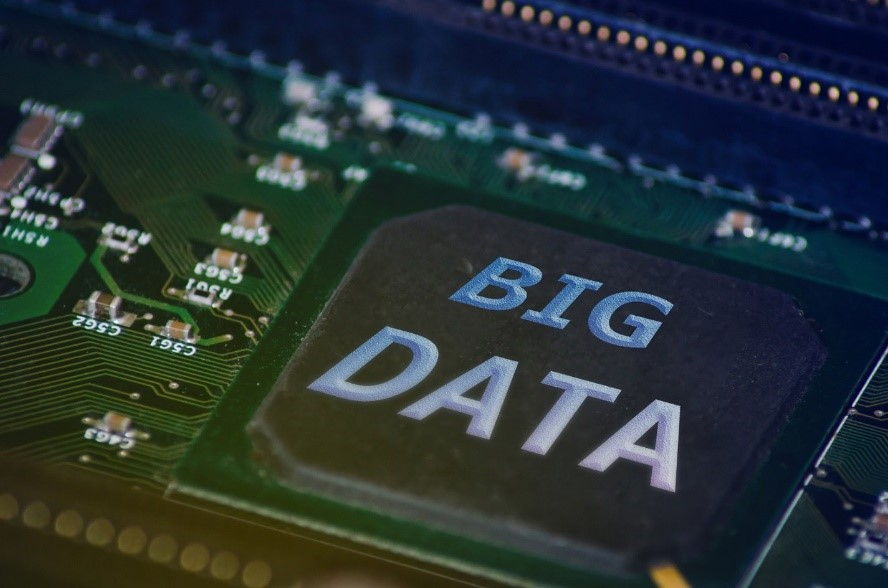
\includegraphics[width=8.5cm]{./Imagenes/img1}
				\end{center}
			\end{figure}
		
			Big Data es un término que describe el gran volumen de datos, tanto estructurados como no estructurados, que inundan los negocios cada día. Pero no es la cantidad de datos lo que es importante. Lo que importa con el Big Data es lo que las organizaciones hacen con los datos. Big Data se puede analizar para obtener ideas que conduzcan a mejores decisiones y movimientos de negocios estratégicos.\cite{bib03:BA:Online} \\ 
			
			¿Porque es tan importarnte este concepto?\\
			
			Lo que hace que Big Data sea tan útil para muchas empresas es el hecho de que proporciona respuestas a muchas preguntas que las empresas ni siquiera sabían que tenían. En otras palabras, proporciona un punto de referencia. Con una cantidad tan grande de información, los datos pueden ser moldeados o probados de cualquier manera que la empresa considere adecuada. Al hacerlo, las organizaciones son capaces de identificar los problemas de una forma más comprensible.\\
			
			La recopilación de grandes cantidades de datos y la búsqueda de tendencias dentro de los datos permiten que las empresas se muevan mucho más rápidamente, sin problemas y de manera eficiente. También les permite eliminar las áreas problemáticas antes de que los problemas acaben con sus beneficios o su reputación.\\
			
			El análisis de Big Data ayuda a las organizaciones a aprovechar sus datos y utilizarlos para identificar nuevas oportunidades. Eso, a su vez, conduce a movimientos de negocios más inteligentes, operaciones más eficientes, mayores ganancias y clientes más felices. Las empresas con más éxito con Big Data consiguen valor de las siguientes formas:\\
			
			\textbf{Reducción de coste}. Las grandes tecnologías de datos, como Hadoop y el análisis basado en la nube, aportan importantes ventajas en términos de costes cuando se trata de almacenar grandes cantidades de datos, además de identificar maneras más eficientes de hacer negocios.\\
			
			\textbf{Más rápido, mejor toma de decisiones.} Con la velocidad de Hadoop y la analítica en memoria, combinada con la capacidad de analizar nuevas fuentes de datos, las empresas pueden analizar la información inmediatamente y tomar decisiones basadas en lo que han aprendido.\\
			
			\textbf{Nuevos productos y servicios.} Con la capacidad de medir las necesidades de los clientes y la satisfacción a través de análisis viene el poder de dar a los clientes lo que quieren. Con la analítica de Big Data, más empresas están creando nuevos productos para satisfacer las necesidades de los clientes.\\
			
							
			\item MACHINE LEARNING 
			
			\begin{figure}[htb]
				\begin{center}
					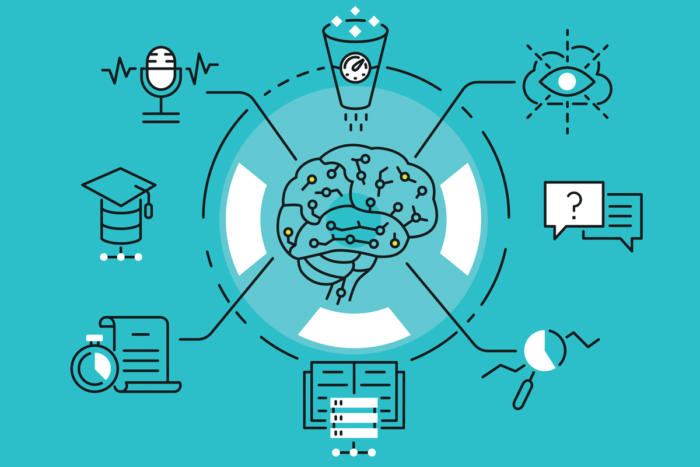
\includegraphics[width=8.41cm]{./Imagenes/img2}
				\end{center}
			\end{figure}
		
			Machine Learning es una disciplina científica del ámbito de la Inteligencia Artificial que crea sistemas que aprenden automáticamente. Aprender en este contexto quiere decir identificar patrones complejos en millones de datos. La máquina que realmente aprende es un algoritmo que revisa los datos y es capaz de predecir comportamientos futuros. Automáticamente, también en este contexto, implica que estos sistemas se mejoran de forma autónoma con el tiempo, sin intervención humana.\cite{bib01:BA:Online} \\
			
			
			El campo de aplicación práctica depende de la imaginación y de los datos que estén disponibles en la empresa. Estos son algunos ejemplos:
			\begin{itemize}
				\item Detectar fraude en transacciones.
				\item Predecir de fallos en equipos tecnológicos.
				\item Prever qué empleados serán más rentables el año que viene (el sector de los Recursos Humanos está apostando seriamente por el Machine Learning).
				\item Seleccionar clientes potenciales basándose en comportamientos en las redes sociales, interacciones en la web…
				\item Predecir el tráfico urbano.
				\item Saber cuál es el mejor momento para publicar tuits, actualizaciones de Facebook o enviar las newsletter.
				\item Hacer prediagnósticos médicos basados en síntomas del paciente.
				\item Cambiar el comportamiento de una app móvil para adaptarse a las costumbres y necesidades de cada usuario.
				\item Detectar intrusiones en una red de comunicaciones de datos.
				\item Decidir cuál es la mejor hora para llamar a un cliente.
				
			\end{itemize}
		
			La tecnología está ahí. Los datos también. ¿Por qué esperar a probar algo que puede suponer una puerta abierta a nuevas formas de tomar decisiones basadas en datos? Seguro que has oído que los datos son el petróleo del futuro. Ahora ya puedes empezar a bombearlo
							
		\end{enumerate}
	
	\newpage
	
	\section{Bussines Intelligence}
	\label{S:2}
	
	BI es un conjunto de técnicas que tienen por finalidad transformar los datos de una empresa en información, identificando posibles indicadores y que estos puedan ser explotados(por ejemplo en cubos), ayudando a la mejora en la toma de decisiones.\\
	
	Nota: Es común confundir que BI solo consiste en la generación cubos, pero ésta es tan solo una parte de toda la arquitectura de BI como se muestra en la figura:
	\begin{figure}[htb]
		\begin{center}
			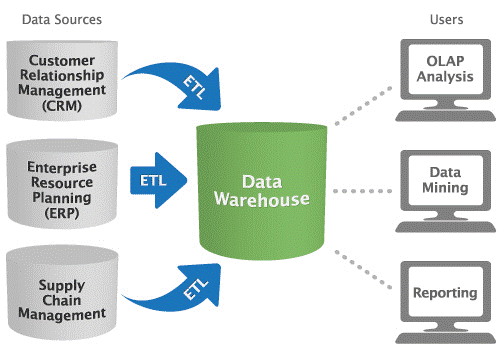
\includegraphics[width=9.5cm]{./Imagenes/img3}
		\end{center}
	\end{figure}
	
	Hasta ahora vamos bien, pero y ¿Qué es Business Analytics?. BA también es un conjunto de técnicas (algoritmos predictivos y modelos estadísticos), pero a diferencia de BI éstas nos permiten predecir posibles resultados (en un futuro), es aquí donde aparecen términos como:Machine Learning, Data Mining, etc.\\
	
	BI nos ayuda a responder preguntas como ¿Quién? ¿Cuándo paso? ¿Qué pasó?, mientras que BA nos ayuda a responder preguntas como ¿Cuándo volverá a suceder?  ¿Quiénes podrían volver a hacerlo?\\
	
	BI se enfoca en toda la data histórica hasta el presente, mostrándote por ejemplo en una empresa como han ido variando sus ventas a lo largo del o de los años, mientras que BA nos permitiría predecir en que mes(futuro) podríamos tener más ventas, teniendo como base los datos históricos que se obtuvieron de BI, es por eso que se puede concluir que estas dos técnicas no son ajenas la una de la otra, sino mas bien son complementarias.\cite{bib01:BI:Online}
		
\end{document}

%%
%% End of file `elsarticle-template-1-num.tex'.
